\documentclass[a4paper, 12pt]{article}
\usepackage[slovene]{babel}
\usepackage[utf8]{inputenc}
\usepackage{lmodern}
\usepackage[T1]{fontenc}
\usepackage{eurosym}
\usepackage{graphicx}

\begin {document}

\begin{center}
{\huge\textbf{Imena}}\\
{\large{Projekt pri predmetu Programiranje 1}}\\
{\large\textsc{Katarina Černe, Neža Dimec}}
\end{center}

\tableofcontents

\newpage

\section{Opis projekta}

Aplikacija, ki je bila ustvarjena pri projektu Imena, omogoča uporabniku, da preko enostavnega iskalnika izbrska nekaj statističnih podatkov o vnešenem imenu:

\begin{itemize}
\item število pojavitev določenega imena v Sloveniji glede na spol,
\item pogostost v Sloveniji,
\end{itemize}

\noindent ter poleg izbrska še podatke o:

\begin{itemize}
\item pomenu imena,
\item izvoru imena,
\item izvorni obliki imena,
\item godovnem dnevu.
\end{itemize}

V primeru, ko se poleg izpisanega rezultata pojavi še *, obstaja možnost, da izpisan rezultat ni najbolj natančen, saj je aplikacija zaradi pomanjkljive spletne baze za vnešeno ime, podatke iskala preko imena, ki je zapisano v izvorni obliki prvotnega imena.

\section{Podatkovni viri}

Vir podatkov sta spletni strani:
\begin{itemize}
\item http://www.stat.si/imena.asp\\
(vir statističnih podatkov)
\item http://sl.wikipedia.org/w/index.php?\\
(vir podatkov o pomenu, izvoru, izvorni obliki, godovnem dnevu)
\end{itemize}

\section{Uporabniški vmesnik z navodili za uporabo}

Uporabnik program zažene tako, da odpre datoteko \texttt{gui\_demo.py}. Ob tem se mu takoj pojavi grafični vmesnik (Slika 1), kamor lahko v iskalno polje vpiše poljubno ime, za katerega bi rad pridobil že omenjene podatke. Ko vpišemo ime, ne pozabimo označiti tudi spola. S klikom na gumb \texttt{Išči!} ali s pritiskom na tipko \texttt{Enter}, se podatki za vpisano ime izpišejo v prikazovalniku spodaj (Slika 2). V primeru, da uporabnik vpiše iskalni niz, ki je neustrezen ali pa se ime v Sloveniji ne pojavlja oz. je njegova pogostost manjša od 5, potem se uporabniku pojavi novo okence, ki ga na to opozori (Slika 3). Ko se iskanja naveličamo, okno enstavno zapremo s klikom na križec desno zgoraj kot ponavadi.

\textsc{Opomba:} Za pravilno delovanje programa morata biti nameščena modula re in requests ter Python 3.4.

\begin{figure}[h]
\centering
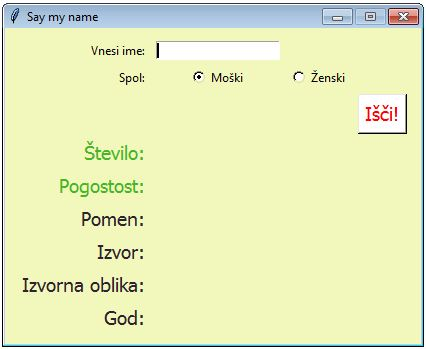
\includegraphics[scale=0.8] {zacetek.jpg}
\caption{Začetno okno.}
\end{figure}

\begin{figure}[h]
\centering
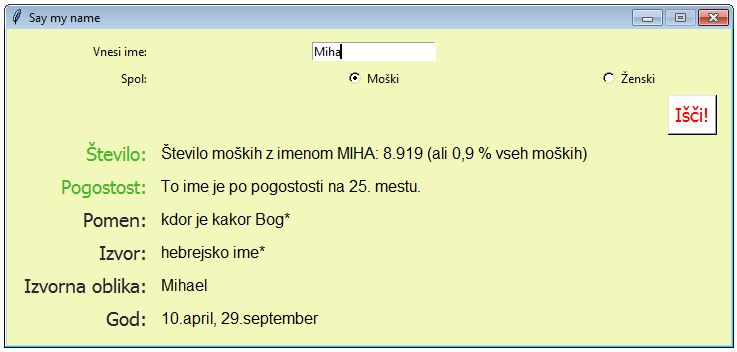
\includegraphics[scale=0.6] {primer.jpg}
\caption{Primer iskanja.}
\end{figure}

\begin{figure}[h]
\centering
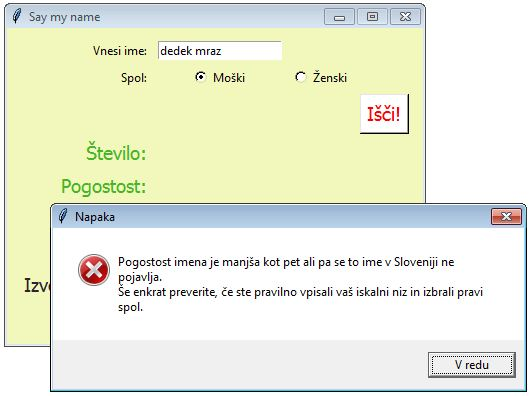
\includegraphics[scale=0.8] {napaka.jpg}
\caption{Izpis napake.}
\end{figure}

\section{Testiranje}
Program za iskanje sva testirali z naključno izbranimi imeni, zato ne izključujeva možnosti, da morda za kakšno izmed imen aplikacija ne prikaže vseh željenih podakov, v primeru, da je stran o imenu iz wikipedije oblikovana kako drugače kot v običajnem primeru. Na primerih, ki sva jih uspeli preizkusiti, aplikacija deluje pravilno.






\end{document}